% =============================================================================
%  Collapse, Convergence, and the Scale of the Prime-Gap Imprint on Polymer Dynamics
%  Merged manuscript: the (unpublished) scale-free Letter + the collapse/convergence paper.
%  Draft 0.1, 1 October 2026.
%
%  DATA PROVENANCE (all CSVs in ../data/)
%   Sec. I   protocol_independence_results.csv, metastability_traces.csv  (Paper 3 repo)
%   Sec. II  s5_scaling_results.csv + s5_scalefree_ext_results.csv   (production ladders)
%            s5_converged_results.csv                                  (32000-step ladders)
%            s6prime_scale_control.csv                                 (S6' ladders, 32000 steps)
%   Sec. III ideal_exact_summary.csv, ideal_exact_retention.csv, ideal_exact_collapse.csv
%            (scripts/ideal_chain_exact.py, NREAL = 40, NBOOT = 2000)
%   Sec. IV  pnt_decoupling_results.csv (production), s5_converged_results.csv +
%            s6prime_scale_control.csv (converged); random_effects_summary.csv
%            (scripts/random_effects_s6prime.py, run 2026-10-01: K=10 x m=5, 1.64 h on 12 workers)
%
%  Figures expected in ./figures/: fig1_protocol.pdf, fig2_metastability.pdf,
%   fig3_globule.pdf (from the collapse paper), fig1_scale_free.pdf (from the Letter,
%   used as Fig. 4), fig5_collapse.pdf (scripts/make_fig_collapse.py).
% =============================================================================
\documentclass[reprint,amsmath,amssymb,aps,pre,longbibliography]{revtex4-2}

\usepackage{graphicx}
\usepackage{bm}
\usepackage{booktabs}
\usepackage[colorlinks=true,linkcolor=blue,citecolor=blue,urlcolor=blue]{hyperref}
\graphicspath{{./figures/}}

\begin{document}

\title{Collapse, Convergence, and the Scale of the Prime-Gap Imprint\\on Polymer Dynamics}

\author{Ruqing Chen}
\email{ruqing@hotmail.com}
\thanks{Archived at \href{https://doi.org/10.5281/zenodo.23076433}{doi:10.5281/zenodo.23076433}.}
\affiliation{GUT Geoservice Inc., Montreal, Quebec, Canada}

\date{\today}

\begin{abstract}
A self-avoiding chain whose bending stiffness is programmed by the prime-gap sequence
(the prime-driven topological polymer, PDTP) collapses into a state that is measurably less
radially sorted than a chain programmed by a random permutation of the same gaps. We settle
two questions about this imprint. First, is it a property of the collapsed state or a memory
of how the chain was cooled? Two independent relaxation routes at $N=4\times10^{4}$,
eight-fold slower annealing and a $10^{6}$-step isothermal hold that drives the chain to a
melt-density globule ($R_g=16.81\pm0.03$, packing fraction $0.489$), converge on the same
nonzero gap, $\Delta\rho_\infty=-0.0269\pm0.0033$ ($8.1\sigma$); the gap is present at every
size from $N=10^{4}$ to $8\times10^{4}$ under the converged protocol. The imprint survives
collapse. Second, what does the size-proportional correlation length $\xi\propto n_{\rm gap}$
of the local-scramble surrogate measure? We show that it measures the readout, not the
primes. A retention-scaling theorem for the exactly solvable ideal chain predicts
$\xi=c\,n_{\rm gap}$ for any readout carried by chain-scale composition, and surrogates that
contain no prime-specific arithmetic (the smooth prime-number-theorem envelope S6$'$ and
the PNT scale family S6$''$) reproduce the proportional law of the true primes, with
$\xi/n_{\rm gap}=0.30$, $0.30$ and $0.33$ for the true, S6$'$ and S6$''$ master curves.
We report the estimator dependence of $\xi$ in the Langevin ensembles, which is as large as
the differences between arms once the arm contrast is small, and replace the single-point
half-crossing by a master-curve collapse in $L/n_{\rm gap}$. The inference from
$\xi\propto n_{\rm gap}$ to extensive arithmetic order in the primes, made in an earlier
unpublished version of this work, is withdrawn. What remains is a smaller, robust statement:
the fold registers the composition of the small-prime end of the chain, of which the smooth
PNT drift supplies a growing fraction ($f_{S6'}=0.25$, $0.34$, $0.57$ at $N=2,4,8\times10^{4}$)
and the discreteness of the small primes supplies the rest; at the sequence level the prime
chain lies below all ten fixed S6$'$ sequences ($Z_{\rm seq}=-3.8$).
\end{abstract}

\maketitle

%==============================================================================
\section{Introduction}
%==============================================================================

The folding of a heteropolymer is governed by its monomer sequence~\cite{deGennes,Pande}.
Periodic sequences drive microphase separation~\cite{Leibler,Bates}; random sequences
produce frustrated, glassy landscapes~\cite{Bryngelson,Garel}. The prime numbers supply a
sequence that is neither: fully deterministic, globally aperiodic, with a logarithmically
decaying density and gap correlations that are neither periodic nor
memoryless~\cite{HardyWright,Cramer,HardyLittlewood}. The prime-driven topological polymer
(PDTP)~\cite{PDTP4} maps the local prime gap onto the local bending stiffness of a
coarse-grained self-avoiding chain, and reads the collapsed conformation through the
Spearman rank correlation $\rho$ between stiffness and radial distance. Against surrogates
that preserve the gap multiset exactly, the true sequence is significantly \emph{less}
radially sorted; the effect is robust at every size, under deeper annealing, and at the
sequence level~\cite{PDTP4}.

Two questions about that imprint were left open by the first version of the model, and an
earlier, unpublished Letter answered one of them wrongly. The first question is whether the
imprint is a property of the collapsed state at all. Every published ensemble was produced by
simulated annealing, which is a kinetic protocol; a chain cooled through a rugged landscape
freezes into whatever basin it reaches, and the basin can depend on the sequence in ways that
have nothing to do with the thermodynamics of the collapsed state. Section~\ref{sec:conv}
tests this objection along two independent relaxation routes and finds that the imprint
survives, at a renormalised amplitude, in a dense globule.

The second question concerns scale. The local-scramble surrogate S5 destroys order within
blocks of $L$ gaps while keeping the blocks in place; the block length at which its retention
of the true signal falls through one half defines a correlation length $\xi$. Measured at four
sizes, $\xi$ grows in proportion to the number of gaps, $\xi\approx0.3\,n_{\rm gap}$. The
Letter read this as ``extensive arithmetic order'' in the primes. Version~4.0 of the PDTP
paper~\cite{PDTP4} proved that this reading does not follow: for the exactly solvable ideal
chain, \emph{any} readout carried by chain-scale structure of the stiffness composition gives
$\xi\propto n_{\rm gap}$, whatever the sequence. Sections~\ref{sec:xi} and~\ref{sec:scale}
make this quantitative. We re-measure $\xi$ at converged depth, report its dependence on the
estimator, and show that two surrogates containing no prime-specific arithmetic reproduce the
proportional law exactly. Section~\ref{sec:pnt} then asks how much of the imprint the smooth
prime-number-theorem (PNT) drift accounts for, and corrects the statistics of that
decomposition for the fact that the prime arm is a single fixed sequence.

The paper therefore supports one physical conclusion and withdraws one inference. The imprint
is real and survives collapse. Its size-proportional correlation length is a property of the
readout, not of the primes.

%==============================================================================
\section{Model and protocols}\label{sec:model}
%==============================================================================

Beads $i=0,\dots,N-1$ are identified with the integers. For a composite bead in the maximal
run of composites bounded by primes $p_{\rm left}<i<p_{\rm right}$ the local gap is
$g_i=p_{\rm right}-p_{\rm left}$; prime beads have $g_i=0$. The gap sets the bending stiffness
through a saturated exponential,
\begin{equation}
k_i=\begin{cases}
\min\!\left[k_{\rm hinge}e^{\alpha g_i},\,k_{\max}\right], & i\ \text{composite},\\[2pt]
k_{\rm hinge}, & i\ \text{prime},
\end{cases}
\label{eq:stiff}
\end{equation}
with $k_{\rm hinge}=0.25$, $\alpha=0.15$, $k_{\max}=500$. Bonds are harmonic
($k_{\rm bond}=45$, $b_0=1$), bending is a cosine potential weighted by
$k_i$~\cite{KratkyPorod,Montesi}, self-avoidance is Weeks--Chandler--Andersen~\cite{WCA}
with the pairwise force capped at $30$, and a weak radial term ($k_{\rm conf}=0.02$) gathers
the globule. Chains are propagated by overdamped Langevin dynamics~\cite{Ermak} in reduced
units ($\sigma=\varepsilon=k_B=\mu=1$, $\Delta t=0.008$, per-bead displacement cap $0.25$)
under geometric annealing from $k_BT=0.50$ to $0.003$~\cite{Kirkpatrick}. The full force
field, parameter table and calibration are given in Ref.~\cite{PDTP4}; nothing is changed
here.

\emph{Surrogates.} All surrogates preserve the exact gap multiset. S1 randomises the order
of the gaps. S5($L$) partitions the ordered gap sequence into contiguous blocks of $L$ gaps,
keeps the blocks in place and randomises the gaps within each block; it interpolates from the
true chain at $L=1$ to S1 at $L\ge n_{\rm gap}=\pi(N)-1$. S6$'$ rank-maps the gaps onto
independent exponential keys of mean $\ln p_k^{\rm smooth}$,
$p_k^{\rm smooth}=k(\ln k+\ln\ln k)$: it reproduces the smooth PNT envelope
$\langle g\rangle\sim\ln i$ and erases every fine correlation. S6$''$ rank-maps the gaps onto
keys $\ln p_k\cdot g'_J$ with $g'_J$ resampled from the global multiset of $g/\ln p$: a pure
PNT scale family~\cite{PDTP4}.

\emph{Observables.} $\rho$ is the Spearman rank correlation between $k_i$ and the radial
distance from the centre of mass; $\Delta R$ is the mean radial distance of the stiffest
$20\%$ of beads minus that of the most flexible $20\%$; $R_g$ is the radius of gyration. The
retention of a surrogate S is
\begin{equation}
f_{\rm S}=\frac{\rho_{\rm S1}-\rho_{\rm S}}{\rho_{\rm S1}-\rho_{\rm true}},
\label{eq:retention}
\end{equation}
unity for a true-like conformation and zero for a shuffle-like one. Unless stated otherwise,
values are ensemble means $\pm$ s.e.m.\ over $n=40$ trajectories per arm, $p$-values are
two-sided Welch tests and $d$ is Cohen's $d$; Sec.~\ref{sec:pnt} supplements these with
sequence-level statistics.

\emph{Protocols.} Three depths occur. The \emph{production} protocol is $5000$, $5000$,
$8000$ and $10^{4}$ annealing steps for $N=1,2,4,8\times10^{4}$ (the depth of the Letter's
ensembles). The \emph{converged} protocol is $32\,000$ steps at every size, the four-fold
deeper anneal at which the ordering gap at $N=4\times10^{4}$ has saturated
(Sec.~\ref{sec:conv}). The \emph{isothermal hold} is $10^{6}$ further steps at $k_BT=0.003$
($\Delta t=0.004$, displacement cap removed) applied to annealed conformations at
$N=4\times10^{4}$.

%==============================================================================
\section{Convergence: the imprint survives collapse}\label{sec:conv}
%==============================================================================

\subsection{Where the production ensemble sits on the collapse pathway}

Held at the final annealing temperature, a production conformation does not sit still. Its
energy falls by $60$--$75\%$ and converges by $\sim\!10^{5}$ steps to a value reached by all
ten trajectories, in both arms, to within $0.3\%$. The rank correlation rises in both arms
and plateaus on the same schedule; fitting $\rho(t)=\rho_\infty-Ae^{-t/\tau}$ gives an
identical relaxation time in the two arms,
$\tau_{\rm relax}=1.68\times10^{4}$ steps $=67\,\tau_{\rm LJ}$, with $\rho_\infty=+0.1635$
(true) and $+0.1935$ (S1). The production anneal at this size spans $64\,\tau_{\rm LJ}$: the
published ensembles were measured after $0.95\,\tau_{\rm relax}$, the hold endpoint after
$60\,\tau_{\rm relax}$.

The relaxed state is a compact, uniform, near-spherical globule (Table~\ref{tab:globule},
Fig.~\ref{fig:globule}a): $R_g=16.81\pm0.03$, flat interior number density
$\simeq1.0\,\sigma^{-3}$, sharp interface at $r\simeq21\,\sigma$, equivalent-sphere packing
fraction $\phi=0.489\pm0.002$, asphericity below $0.06$, identical in the two arms. The ten
independent endpoints agree in $R_g$ to two parts in a thousand. The representative
production conformation of the first PDTP paper, by contrast, has $R_g\approx111$: a
partially collapsed coil at $\sim10^{-3}$ of globule density. The earlier work measured the
imprint on the collapse \emph{pathway}, not at its end.

\begin{table}[b]
\caption{Structure of the relaxed globule at the end of the $10^{6}$-step hold
($N=4\times10^{4}$, five endpoints per arm, mean $\pm$ s.d.). $R_{\rm eff}=R_g\sqrt{5/3}$,
$\phi$ is the packing fraction of $\sigma$-diameter beads in the equivalent sphere,
$z_{\rm nb}$ the mean number of non-bonded neighbours within $2^{1/6}\sigma$.}
\label{tab:globule}
\footnotesize
\begin{ruledtabular}
\begin{tabular}{lccccc}
arm & $R_g$ & $R_{\rm eff}$ & $\phi$ & $z_{\rm nb}$ & asphericity\\ \hline
true & $16.82\pm0.02$ & $21.71\pm0.03$ & $0.489\pm0.002$ & $3.39$ & $0.045\pm0.011$\\
S1   & $16.80\pm0.03$ & $21.68\pm0.04$ & $0.490\pm0.003$ & $3.40$ & $0.041\pm0.009$\\
\end{tabular}
\end{ruledtabular}
\end{table}

\subsection{Protocol independence: the gap renormalises, then saturates}

Slowing the anneal by factors of $2$, $4$ and $8$ ($n=40$ per arm per protocol) moves the
ordering gap and then stops moving (Table~\ref{tab:stageB}, Fig.~\ref{fig:protocol}).
Between $1\times$ and $4\times$ the gap shrinks by $42\%$, from $-0.0457$ to $-0.0263$;
between $4\times$ and $8\times$ it does not shrink at all ($-0.0263$ versus $-0.0262$,
constant-gap $\chi^{2}=0.00/1$). A saturating fit
$\Delta\rho=\Delta\rho_\infty+Ae^{-x/\tau}$ in $x=\log_2(\text{protocol})$ gives
$\Delta\rho_\infty=-0.0254\pm0.0061$. The gap is significant at every protocol
(Welch $p\le6.4\times10^{-6}$), and its effect size is stable across the converged protocols
($d=-1.15$, $-1.10$, $-1.16$).

\begin{table}[t]
\caption{Ordering gap versus annealing length at $N=4\times10^{4}$, $n=40$ per arm per
protocol; s.e.m.\ in parentheses on the last digits. The $1\times$ row is the production
ensemble.}
\label{tab:stageB}
\footnotesize
\begin{ruledtabular}
\begin{tabular}{rcccc}
steps & $\rho_{\rm true}$ & $\rho_{\rm S1}$ & $\Delta\rho$ & $d$\\ \hline
$8\,000$ ($1\times$)  & $+0.0942(65)$ & $+0.1399(34)$ & $-0.0457(73)$ & $-1.39$\\
$16\,000$ ($2\times$) & $+0.1506(56)$ & $+0.1822(24)$ & $-0.0315(61)$ & $-1.15$\\
$32\,000$ ($4\times$) & $+0.1659(46)$ & $+0.1922(27)$ & $-0.0263(53)$ & $-1.10$\\
$64\,000$ ($8\times$) & $+0.1563(36)$ & $+0.1825(35)$ & $-0.0262(51)$ & $-1.16$\\
\end{tabular}
\end{ruledtabular}
\end{table}

\begin{figure}[t]
\centering
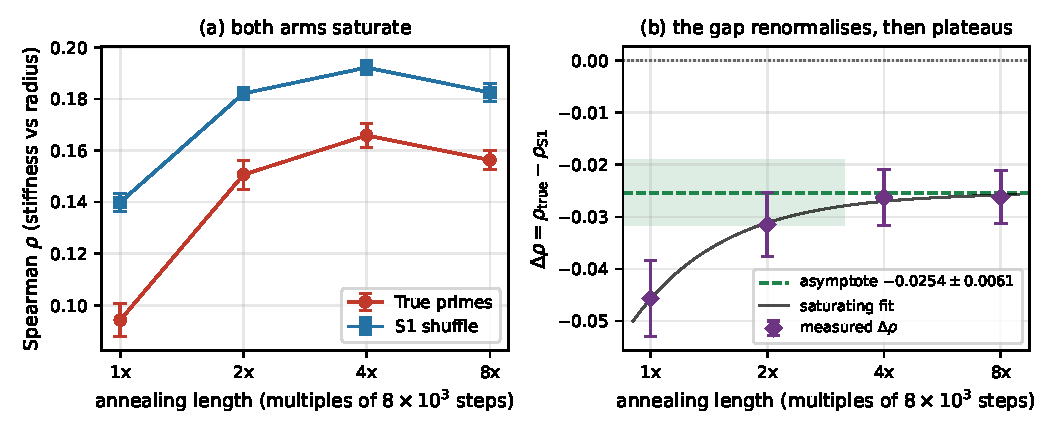
\includegraphics[width=\linewidth]{fig1_protocol.pdf}
\caption{Protocol independence at $N=4\times10^{4}$. (a)~Both arms converge: $\rho$ rises
from the production protocol and saturates by $4\times$. (b)~The ordering gap renormalises
downward by $42\%$ between $1\times$ and $4\times$ and is then constant; green band: the
asymptote of the saturating fit.}
\label{fig:protocol}
\end{figure}

\subsection{Isothermal metastability}

Over the hold, $\rho$ rises by $+0.0147$ (true) and $+0.0090$ (S1), both significant against
zero at $n=5$: the production measurement is taken mid-relaxation. But the drift is the
approach to a plateau reached well inside the hold (Fig.~\ref{fig:meta}). Beyond
$10^{5}$ steps ($6\,\tau_{\rm relax}$) the energy is constant to $0.2\%$, the ensemble-mean
$\rho$ moves by less than $0.004$ in either arm, and the gap settles at
\begin{equation}
\Delta\rho\big|_{\rm hold}=-0.0299\pm0.0077,
\end{equation}
flat to $0.9\%$ of its own value over the final $90\%$ of the hold ($p=0.0067$, $d=-2.46$ at
$n=5$). Relaxation homogenises the ensemble (the between-run s.d.\ of $\rho$ falls threefold)
while preserving trajectory identity (Pearson $r=0.91$ between initial and final $\rho$): a
near-uniform shift of the whole ensemble, not a re-randomisation.

\begin{figure}[t]
\centering
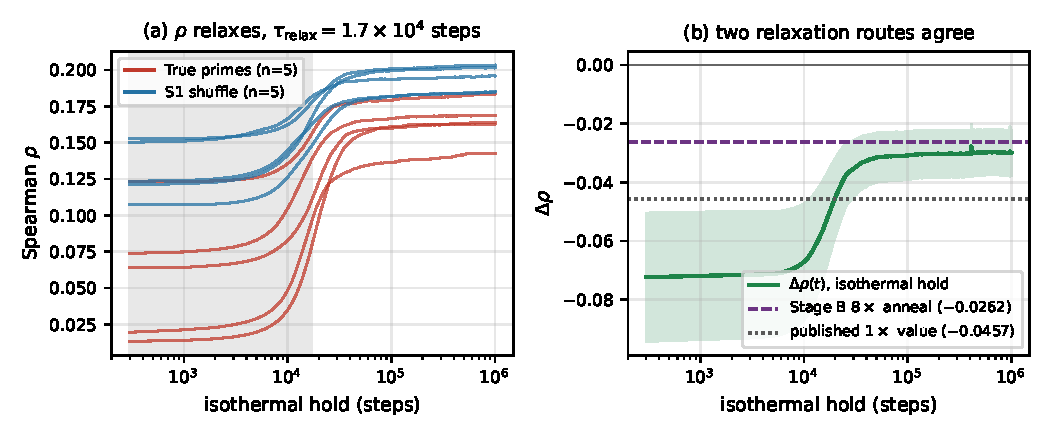
\includegraphics[width=\linewidth]{fig2_metastability.pdf}
\caption{Isothermal hold at $k_BT=0.003$, $N=4\times10^{4}$, $n=5$ per arm, $10^{6}$ steps.
(a)~Individual $\rho$ traces; both arms relax with $\tau_{\rm relax}=1.68\times10^{4}$ steps
(shaded). (b)~The ordering gap shrinks during the relaxation and is then flat; its plateau
coincides with the independently obtained $8\times$-anneal value (dashed).}
\label{fig:meta}
\end{figure}

\subsection{The converged amplitude}

The two routes are mechanistically distinct (slower cooling versus isothermal ageing; capped
versus uncapped propagator; $n=40$ versus $n=5$) and they agree ($z=0.40$, $p=0.69$).
Combining the three converged estimates,
\begin{equation}
\Delta\rho_\infty=-0.0269\pm0.0033\qquad(8.1\sigma),\qquad\chi^{2}=0.18/2.
\label{eq:combined}
\end{equation}
This is $59\%$ of the production value: two-fifths of the published separation was incomplete
relaxation. Under the converged ($32\,000$-step) protocol the gap is present at every size
(Table~\ref{tab:convsizes}): $\Delta\rho=-0.026$, $-0.039$, $-0.038$, $-0.041$ for
$N=1,2,4,8\times10^{4}$, all at $p\le3\times10^{-4}$. The core--shell amplitude $\Delta R$,
by contrast, does not survive collapse: it falls from $\simeq14$ to $2.6\,\sigma$ as the
globule compacts and the arm difference ($-0.24\,\sigma$, $p=0.14$) is unresolved
(Fig.~\ref{fig:globule}b). In a globule whose density profile is flat out to a sharp
interface there is little radial room for the stiffness extremes to separate; the rank
estimator, which uses the whole distribution, retains its resolving power.

\begin{table}[t]
\caption{Ordering gap at the converged protocol ($32\,000$ steps, $n=40$ per arm) at four
sizes, from the same ensembles as the S5 ladders of Sec.~\ref{sec:xi}.}
\label{tab:convsizes}
\begin{ruledtabular}
\begin{tabular}{lcccc}
$N$ & $\rho_{\rm true}$ & $\rho_{\rm S1}$ & $\Delta\rho$ & $p$\\ \hline
$1\times10^{4}$ & $+0.0774$ & $+0.1037$ & $-0.0263$ & $2.9\times10^{-4}$\\
$2\times10^{4}$ & $+0.1074$ & $+0.1460$ & $-0.0386$ & $7.3\times10^{-9}$\\
$4\times10^{4}$ & $+0.1602$ & $+0.1982$ & $-0.0380$ & $8.6\times10^{-10}$\\
$8\times10^{4}$ & $+0.1978$ & $+0.2388$ & $-0.0411$ & $8.2\times10^{-17}$\\
\end{tabular}
\end{ruledtabular}
\end{table}

\begin{figure}[t]
\centering
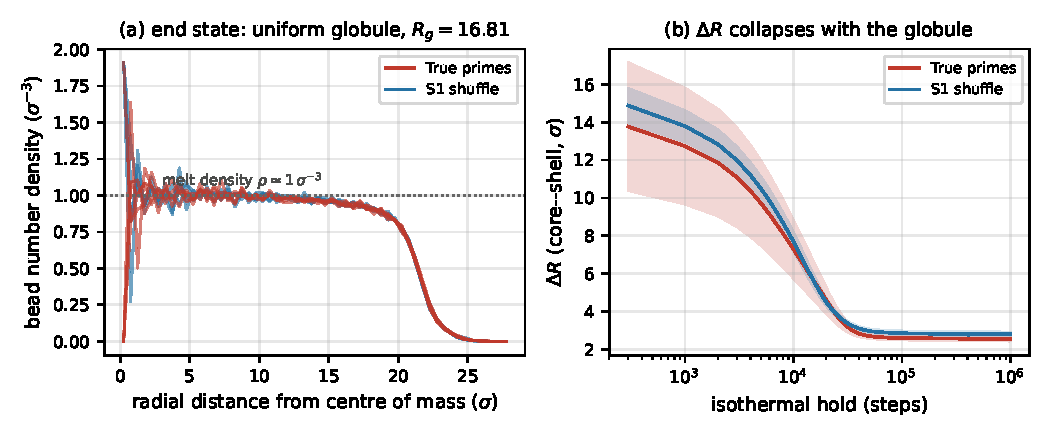
\includegraphics[width=\linewidth]{fig3_globule.pdf}
\caption{The relaxed state. (a)~Radial bead-density profiles of the ten endpoint
configurations: a uniform interior at melt density with a sharp interface at
$r\simeq21\,\sigma$, identical in both arms. (b)~The core--shell amplitude $\Delta R$
collapses with the globule and no longer separates the arms.}
\label{fig:globule}
\end{figure}

The kinetic-artefact objection is thus answered in the direction the model needed. A frozen
memory of cooling would decay monotonically as cooling slows and would not survive a
five-fold contraction of the chain and a $70\%$ drop in energy. This gap decays by $42\%$ and
then stops, and survives both. Neither route is equilibrium sampling, which is out of reach
at these sizes (the production force field is non-conservative through its force and
displacement caps, and a replica-exchange ladder at $N=4\times10^{4}$ would need
$\sim10^{3}$ replicas); what is established is protocol independence of a converged,
compacted state along two independent routes.

%==============================================================================
\section{The correlation length and its estimator}\label{sec:xi}
%==============================================================================

\subsection{Definition and the production measurement}

The S5 local scramble measures the scale over which the ordering signal survives. Its
retention $f(L)$ [Eq.~\eqref{eq:retention}] falls from unity at small $L$ to zero at
$L\ge n_{\rm gap}$, and the block length at which it falls through one half defines $\xi$.
Operationally, in the Letter and here, $\xi$ is the last downward crossing of $f(L)$ through
$1/2$, located by linear interpolation in $\log L$; its uncertainty is a $68\%$ percentile
interval from $8000$ bootstrap resamples of the per-trajectory $\rho$ values in every arm,
with the crossing construction repeated on each resample.

At the production protocol (Table~\ref{tab:xi}, Fig.~\ref{fig:scaling}) the correlation
length grows with the sequence: a $6.4$-fold increase in $n_{\rm gap}$ produces a $5.0$-fold
increase in $\xi$. A single-parameter proportional law fits the four points
($\chi^{2}=1.93/3$) and a fixed length is rejected ($\chi^{2}=10.45/3$, $p=0.015$). The
ratio $\xi/n_{\rm gap}$ lies between $0.26$ and $0.39$.

\begin{table*}[t]
\caption{The S5 half-retention length at the production protocol ($5000/5000/8000/10^{4}$
steps for $N=1,2,4,8\times10^{4}$, $n=40$ per arm) with $68\%$ bootstrap intervals, and at
the converged protocol ($32\,000$ steps at every size) with two estimators. LC: last
downward crossing of $f(L)$ through $1/2$; LG: half-point of a three-parameter logistic fit
to $f(\ln L)$ (Appendix~\ref{app:est}). At $N=8\times10^{4}$ under the converged protocol
the retention stays near one half across the whole ladder ($f=0.38$--$0.57$ for
$L=50$--$2299$) and the LC estimate is not determined (its bootstrap interval spans
$[386,2490]$).}
\label{tab:xi}
\begin{ruledtabular}
\begin{tabular}{lccccc}
 & & \multicolumn{1}{c}{production} & \multicolumn{2}{c}{converged} \\
$N$ & $n_{\rm gap}$ & $\xi$ (LC) & $\xi$ (LC) & $\xi$ (LG) & \\ \hline
$1\times10^{4}$ & $1228$ & $482\ [406,574]$   & $415\ [362,464]$   & $364$  &\\
$2\times10^{4}$ & $2261$ & $766\ [550,1031]$  & $668\ [249,902]$   & $1176$ &\\
$4\times10^{4}$ & $4202$ & $1086\ [757,1346]$ & $1774\ [1526,2060]$& $2182$ &\\
$8\times10^{4}$ & $7836$ & $2407\ [1320,2869]$& undetermined       & $3940$ &\\ \hline
$\xi/n_{\rm gap}$ & & $0.39,0.34,0.26,0.31$ & $0.34,0.30,0.42,-$ & $0.30,0.52,0.52,0.50$ &\\
\end{tabular}
\end{ruledtabular}
\end{table*}

\begin{figure}[t]
\centering
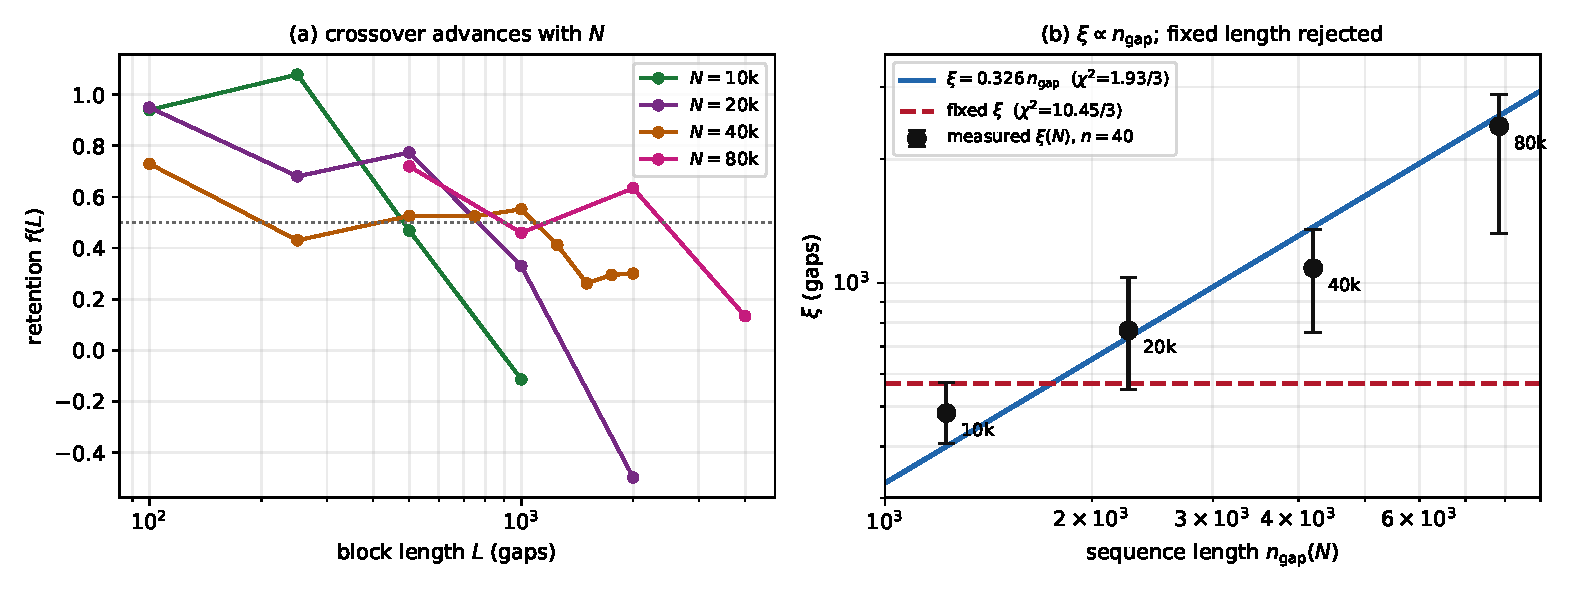
\includegraphics[width=\linewidth]{fig1_scale_free.pdf}
\caption{Production-protocol measurement. (a)~Retention $f(L)$ of the S5 local scramble at
four sizes, $n=40$ per point (mean $\pm$ s.e.m.); the half-retention crossover (dotted)
advances toward larger block length as the sequence grows. (b)~$\xi$ against $n_{\rm gap}$
with $68\%$ bootstrap intervals; solid: proportional law; dashed: best fixed length. This
apparent growth was interpreted in earlier work as arithmetic order; Fig.~\ref{fig:collapse}
and Sec.~\ref{sec:scale} show it is reproduced by non-arithmetic surrogates.}
\label{fig:scaling}
\end{figure}

\subsection{The converged measurement and the estimator problem}

Re-measured at the converged protocol with the same estimator (Table~\ref{tab:xi}, columns
LC), $\xi$ remains macroscopic and a fixed length remains rejected
($\chi^{2}=25/3$), but the ratios change: $0.34$, $0.30$, $0.42$ at $N=1,2,4\times10^{4}$,
and at $N=8\times10^{4}$ the retention stays close to one half from the smallest block
($L=50$, $f=0.38$) to $L=2299$ ($f=0.47$) before falling, so that no half-crossing can be
assigned. The dependence on protocol at fixed $N$ is not monotone: at $N=10^{4}$,
$\xi=350$, $482$ and $415$ gaps after $2000$, $5000$ and $32\,000$ steps; at
$N=2\times10^{4}$ deeper annealing lowers $\xi$, at $4\times10^{4}$ it raises it. The
Letter's argument that the protocol bias is ``conservative'' because $\xi$ increases with
depth is therefore unsupported and is withdrawn.

A second estimator, the half-point of a logistic fit to $f(\ln L)$ with free amplitude,
width and centre (the estimator of the converged-ladder driver, Appendix~\ref{app:est}),
gives $0.30$, $0.52$, $0.52$, $0.50$ on the same data. The two estimators agree at
$N=10^{4}$ and disagree by up to a factor two elsewhere; neither is wrong, because the
retention curves at converged depth are not monotone, and a single half-point of a
non-monotone curve is not well defined.

The problem is sharpest where the arm contrast is small. Applying the S5 ladder to S6$'$
(Sec.~\ref{sec:scale}), the denominator of Eq.~\eqref{eq:retention} is
$\rho_{\rm S1}-\rho_{\rm S6'}=0.010$--$0.023$ against a per-point s.e.m.\ of
$\rho_{\rm S5}$ of $\simeq0.005$: $f(L)$ then carries errors of $0.3$--$0.5$ per point, takes
values up to $1.8$, and crosses one half several times. For these ladders the LC estimator
gives $\xi/n_{\rm gap}=0.43$, $0.61$, $0.58$ and the LG estimator $0.15$, $0.15$, $0.27$. A
Langevin measurement of $\xi$ on a weak arm is therefore not a number but a range, and we
report it as such.

We adopt two remedies. First, within the Langevin data we replace the single-point crossing
by the \emph{master-curve collapse}: $f$ is plotted against $L/n_{\rm gap}$ for all sizes,
and the statement tested is whether the curves coincide (Sec.~\ref{sec:scale},
Fig.~\ref{fig:collapse}c). Second, the decisive comparison between arms is made in the
exact ideal-chain readout, where there is no thermal noise and the only variance is that of
the surrogate construction.

%==============================================================================
\section{The scale is a property of the readout}\label{sec:scale}
%==============================================================================

\subsection{The retention-scaling theorem}

Reference~\cite{PDTP4} solves the ideal (phantom) chain with the quenched PDTP bending field
exactly: the thermally averaged radial profile $P_i=\langle|\mathbf r_i-\mathbf r_{\rm cm}|^2\rangle$
of any sequence follows from the tangent-product formula
$\langle\mathbf t_a\cdot\mathbf t_b\rangle=\prod_{k=a+1}^{b}\mathcal L(\beta k_k)$ in
$O(N)$ operations. For a homogeneous chain $P_i$ reduces to the classical end-to-middle
U-shaped profile; the ends lie peripherally as a positional fact. The ideal readout
$\rho_{\rm id}={\rm Spearman}(k_i,P_i)$ isolates the positional channel: how the
composition of the sequence is distributed relative to the chain ends.

Let $m_i=\phi(k_i)-\bar\phi$ be the composition field ($\phi$ the rank transform, identical
across multiset-preserving arms). A readout is \emph{chain-scale} if its arm contrast depends
on the sequence through projections $\langle m,F\rangle=\sum_i m_iF(i/N)$ on functions of
bounded variation. Theorem~1 of Ref.~\cite{PDTP4} states that under S5 with blocks of $L$
gaps,
\begin{equation}
\big|\langle m-\bar m_L,F\rangle\big|\le\frac{L\bar g}{N}\,{\rm TV}(F)\,\|m\|_\infty ,
\label{eq:tv}
\end{equation}
with $\bar m_L$ the block average, so that the retention depends on $L/n_{\rm gap}$ alone
(up to the slow variation of the mean gap $\bar g$) and its half-point is
$\xi=c_F\,n_{\rm gap}$. The constant $c_F$ is fixed by the shape of $F$ and the chain-scale
content of $m$; it is not an arithmetic quantity. A monotone PNT drift, which spans the
whole sequence by construction, is a chain-scale composition profile and therefore
suffices. The theorem also permits $\ln n_{\rm gap}$ corrections through $\bar g$, which
is why the Letter's distinction between a strictly proportional and a log-corrected law has
no content and is not pursued here.

\subsection{Surrogates without arithmetic reproduce the proportional law}

The theorem predicts that S6$'$ and S6$''$, which carry the PNT envelope and nothing
prime-specific, give the same $\xi/n_{\rm gap}$ as the primes. We test this in the exact
readout at four sizes (\texttt{ideal\_chain\_exact.py}: $40$ realisations of every
surrogate per block length, $2000$ bootstrap resamples; Table~\ref{tab:exact},
Fig.~\ref{fig:collapse}a,b). Every arm has a negative contrast against S1 ($z=-1.4$ to
$-3.3$) and a macroscopic, size-proportional $\xi$. The size-averaged master curves have
half-points
\begin{equation}
\frac{\xi}{n_{\rm gap}}=0.30\ (\text{true}),\quad 0.30\ (\text{S6}'),\quad 0.33\ (\text{S6}''),
\end{equation}
and the r.m.s.\ spread of $f$ across the four sizes on a common $L/n_{\rm gap}$ grid is
$0.08$--$0.12$ for all three arms. The per-size values scatter ($0.21$--$0.40$), and the
S6$'$ half-points at $N=1$ and $2\times10^{4}$ ($0.23$, $0.21$) lie below the true value.
Two effects, both finite-size, account for this. First, the S6$'$ contrast against S1 is
smallest at small $N$ ($z=-1.4$), so the denominator of Eq.~\eqref{eq:retention} is small
and the single-size half-point inherits the full construction variance of the ensemble,
exactly as in the Langevin ladders. Second, the bound of Eq.~\eqref{eq:tv} is not
uniform in $N$: its right-hand side carries the mean gap $\bar g$ and the total variation of
the readout profile, and at $N=10^{4}$ the small-prime region, where $\ln p_i$ rises in
discrete steps and the gap law is far from a scale family, is a larger fraction of the chain
than at $8\times10^{4}$. The constant $c_F$ therefore approaches its asymptotic value only as
the chain-end composition becomes a vanishing fraction of the backbone, and S6$'$, which
replaces the discrete small-prime gaps by a smooth envelope, converges from below. Once the
curves are normalised to $L/n_{\rm gap}$ and averaged over sizes these effects cancel: the
master-curve half-points of the true primes and of S6$'$ coincide ($0.30$ versus $0.30$),
and the proportional law and its coefficient are the same for the true primes and for the
two surrogates that contain no prime-specific arithmetic. This is the result the
theorem requires and the result the Letter's inference cannot survive: the growth of $\xi$
with $n_{\rm gap}$, and its coefficient, are produced by the smooth PNT envelope read
through the end-to-middle profile.

\begin{table*}[t]
\caption{Exact ideal-chain readout: half-retention length of the S5 scramble applied to
the true primes, to S6$'$ and to S6$''$ ($40$ realisations per point, $68\%$ bootstrap
intervals over the surrogate ensemble; the true arm is one fixed sequence). $z$ is the
contrast of the top arm against the S1 ensemble in units of the S1 s.d. Last row: half-point
of the size-averaged master curve in $L/n_{\rm gap}$.}
\label{tab:exact}
\begin{ruledtabular}
\begin{tabular}{lccccccc}
 & \multicolumn{2}{c}{true} & \multicolumn{2}{c}{S6$'$} & \multicolumn{2}{c}{S6$''$}\\
$N$ & $z$ & $\xi/n_{\rm gap}$ & $z$ & $\xi/n_{\rm gap}$ & $z$ & $\xi/n_{\rm gap}$ \\ \hline
$1\times10^{4}$ & $-2.4$ & $0.33\ [0.29,0.40]$ & $-1.4$ & $0.23\ [0.20,0.30]$ & $-1.7$ & $0.40\ [0.34,0.43]$\\
$2\times10^{4}$ & $-1.6$ & $0.29\ [0.28,0.31]$ & $-1.4$ & $0.21\ [0.19,0.37]$ & $-1.8$ & $0.31\ [0.26,0.36]$\\
$4\times10^{4}$ & $-2.5$ & $0.33\ [0.31,0.35]$ & $-2.2$ & $0.35\ [0.32,0.39]$ & $-1.9$ & $0.27\ [0.23,0.31]$\\
$8\times10^{4}$ & $-3.1$ & $0.27\ [0.25,0.28]$ & $-2.4$ & $0.31\ [0.28,0.34]$ & $-3.3$ & $0.34\ [0.32,0.37]$\\ \hline
master curve & & $0.30$ & & $0.30$ & & $0.33$\\
\end{tabular}
\end{ruledtabular}
\end{table*}

\begin{figure*}[t]
\centering
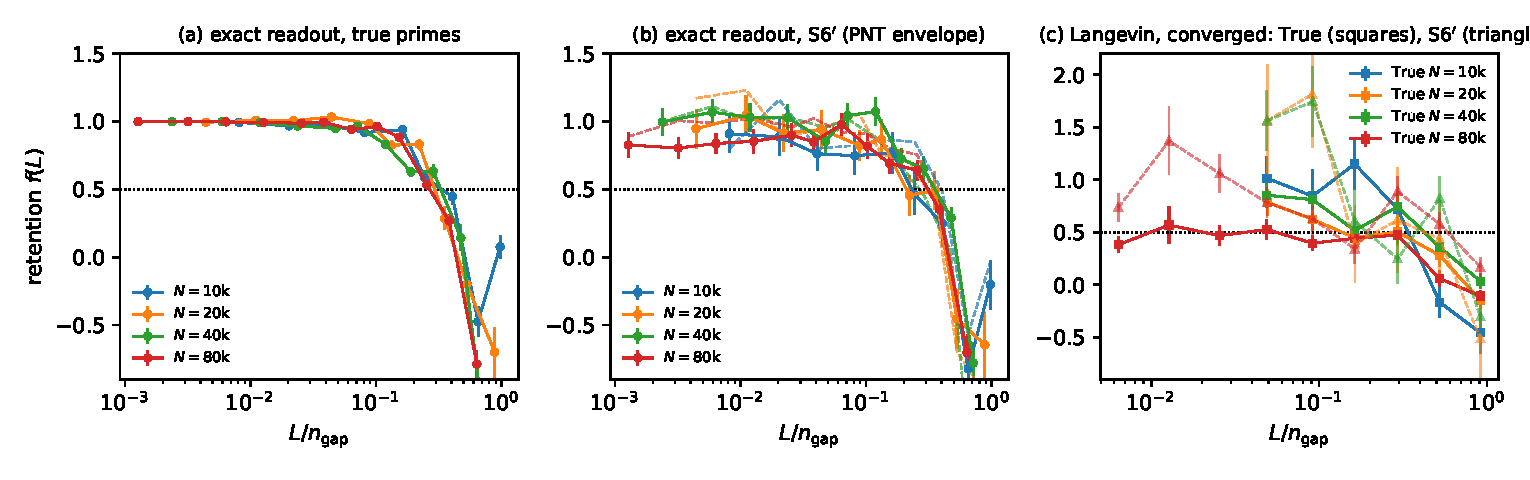
\includegraphics[width=\linewidth]{fig5_collapse.pdf}
\caption{Retention against $L/n_{\rm gap}$. (a)~Exact ideal-chain readout, true primes at
four sizes (error bars: bootstrap s.d.\ over the S1 and S5 ensembles). (b)~Same for S6$'$
(symbols) and S6$''$ (dashed): the surrogates without prime-specific arithmetic collapse
onto the same master curve as the primes. (c)~Langevin ensembles at the converged protocol:
true (squares) and S6$'$ (triangles). The true curves collapse to within their errors; the
S6$'$ curves are dominated by the small arm contrast (Sec.~\ref{sec:xi}).}
\label{fig:collapse}
\end{figure*}

In the Langevin ensembles the same collapse holds for the true primes within their errors
(Fig.~\ref{fig:collapse}c): the converged curves at $N=1$, $2$ and $4\times10^{4}$ lie on one
band in $L/n_{\rm gap}$, and the $8\times10^{4}$ curve lies below it at small blocks, where a
partial loss of retention already at $L=50$ is not captured by the ideal readout. We return
to this point, which we read as a finite-depth kinetic effect, in Sec.~\ref{sec:disc}. The Langevin S6$'$ ladders, run at $N=2,4,8\times10^{4}$ under the converged protocol,
also show a retention that moves toward larger $L$ as the sequence grows, but their small
contrast makes the curves too noisy to locate a half-point reliably; we therefore rest the
quantitative statement on the exact readout, where the point is settled without noise.

\subsection{What is withdrawn}

The Letter inferred, from $\xi\propto n_{\rm gap}$, that ``the arithmetic order the fold
registers is extensive'' and that the primes carry ``scale-free long-range order'' visible
to the fold. That inference is withdrawn, together with the fixed coefficient $0.326$ (the
measured ratio depends on protocol and estimator and lies in the range $0.27$--$0.37$ for
the true primes at converged depth and in the exact readout), the claim that the protocol
bias is conservative, and the discussion of a logarithmic correction. The Letter's
conjecture that the fold registers the hyperuniform, limit-periodic order of the
primes~\cite{Torquato2018,Torquato2019} is not supported either: Ref.~\cite{PDTP4} shows
that spectrum-matched IAAFT surrogates reproduce most of the effect and that the
small-wavenumber hyperuniform exponent of the sequence is not transmitted to the
scattering function at all.

%==============================================================================
\section{The PNT share and the residual}\label{sec:pnt}
%==============================================================================

\subsection{Decomposition at production and at converged depth}

Macroscopic order in the gap sequence has two layers: the smooth PNT drift of the mean gap,
$\langle g_i\rangle\sim\ln i$, and the deterministic fluctuation riding on it. S6$'$
carries the first and not the second, so $f_{S6'}$ [Eq.~\eqref{eq:retention}] is the
fraction of the ordering effect reproduced by the envelope alone
(Table~\ref{tab:pnt}). At the production protocol it is $0.32$ and $0.44$ at
$N=2$ and $4\times10^{4}$. At the converged protocol it is $0.25$, $0.34$ and $0.57$ at
$N=2$, $4$ and $8\times10^{4}$: the share of the smooth envelope grows with $N$, as a drift
that spans the whole chain should, while the residual true$-$S6$'$ gap remains significant
at every size ($p\le10^{-4}$) and shrinks in absolute terms from $-0.029$ to $-0.018$.

\begin{table*}[t]
\caption{PNT decomposition. $f_{S6'}=(\rho_{\rm S1}-\rho_{S6'})/(\rho_{\rm S1}-\rho_{\rm true})$,
$n=40$ per arm; $p$ and $d$ refer to the true$-$S6$'$ contrast (Welch, fresh S6$'$ sequence
per trajectory). For the converged $N=2\times10^{4}$ row the sequence-level design of
Sec.~\ref{sec:re} (Table~\ref{tab:re}) gives $Z_{\rm seq}=-3.75$, $p=4.6\times10^{-3}$, and
$f_{S6'}=0.46\ [0.32,0.59]$ with fixed S6$'$ sequences.}
\label{tab:pnt}
\begin{ruledtabular}
\begin{tabular}{llccccc}
protocol & $N$ & $\rho_{\rm true}$ & $\rho_{S6'}$ & $\rho_{\rm S1}$ & $f_{S6'}$ & true$-$S6$'$ ($p$, $d$)\\ \hline
production & $2\times10^{4}$ & $+0.0396$ & $+0.0654$ & $+0.0777$ & $0.32$ & $-0.0258$ ($3.8\times10^{-2}$, $-0.47$)\\
production & $4\times10^{4}$ & $+0.0942$ & $+0.1197$ & $+0.1399$ & $0.44$ & $-0.0254$ ($4.0\times10^{-3}$, $-0.66$)\\
converged  & $2\times10^{4}$ & $+0.1074$ & $+0.1364$ & $+0.1460$ & $0.25$ & $-0.0291$ ($8.9\times10^{-6}$, $-1.06$)\\
converged  & $4\times10^{4}$ & $+0.1602$ & $+0.1851$ & $+0.1982$ & $0.34$ & $-0.0250$ ($1.3\times10^{-5}$, $-1.04$)\\
converged  & $8\times10^{4}$ & $+0.1978$ & $+0.2155$ & $+0.2388$ & $0.57$ & $-0.0177$ ($5.2\times10^{-5}$, $-0.96$)\\
\end{tabular}
\end{ruledtabular}
\end{table*}

Two cautions from Ref.~\cite{PDTP4} apply. S6$'$ reproduces only $50$--$80\%$ of the true
chain-scale composition (the leading Legendre coefficients of ${\rm rank}(k_i)$), so
$1-f_{S6'}$ is an upper bound on the non-PNT share. The improved scale family S6$''$, which
reproduces those coefficients to $0.93$--$1.0$ and recovers the full effect in the ideal
readout, was predicted to give $f\approx1$ in the Langevin model and gave $0.62\ [0.38,0.94]$
at $N=2\times10^{4}$ and $0.28\ [0.11,0.45]$ at $4\times10^{4}$ (production protocol). A
smooth model of the composition does not reproduce the effect in the interacting globule.

\subsection{Where the residual lives}

Reference~\cite{PDTP4} locates the residual directly: restricting the Spearman readout to
bead subsets, the true$-$S1 gap at $N=4\times10^{4}$ is $-0.045$ on the whole chain, $-0.018$
with the first $5\%$ of beads excluded and $+0.002$ ($p=0.89$) with the first $10\%$ excluded,
in both production and isothermally relaxed ensembles; the two halves carry opposite signs
of the form the positional readout predicts. The true$-$S6$''$ residual is likewise
concentrated at the start ($-0.027$ overall, $-0.013$ with the first $10\%$ excluded). The
fold reads the composition of the small-prime end of the chain, where the PNT drift is
steepest and the gaps are short and regular. The smooth envelope accounts for a growing
fraction of this as $N$ increases (Table~\ref{tab:pnt}); the rest is the discreteness of the
small primes, which no $\ln p$-scaled model reproduces.

\subsection{Sequence-level statistics}\label{sec:re}

The true arm is one fixed sequence, while every S6$'$ and S1 trajectory above drew a fresh
surrogate sequence. Writing $\rho=\mu+s+\varepsilon$ with a sequence effect $s$ of variance
$\sigma^{2}_{\rm seq}$ and thermal noise $\varepsilon$, the variance of
$\bar\rho_{\rm true}-\bar\rho_{\rm S}$ under the null ``the primes are a typical member of
the class S'' contains $\sigma^{2}_{\rm seq}$, which does not shrink with $n$ and which the
Welch statistic omits~\cite{PDTP4}. For the shuffle class at $N=10^{4}$ the omitted term is
undetectable next to thermal noise (ANOVA $p=0.95$; the prime chain lies below all twelve
fixed shuffles, $Z_{\rm seq}=-7.0$)~\cite{PDTP4}. For the S6$'$ class it has not been
measured. We therefore run $K=10$ fixed S6$'$ sequences with $m=5$ trajectories each at
$N=2\times10^{4}$ under the converged protocol (\texttt{random\_effects\_s6prime.py}), and
report
\begin{equation}
Z_{\rm seq}=\frac{\bar\rho_{\rm true}-\hat\mu}{\sqrt{\hat\sigma^{2}_{\rm seq}+s^{2}_{\rm true}/n_{\rm true}+{\rm Var}\,\hat\mu}},
\label{eq:zseq}
\end{equation}
\begin{equation}
{\rm Var}\,\hat\mu=\frac{\hat\sigma^{2}_{\rm seq}+\hat\sigma^{2}_{\rm th}/m}{K},
\end{equation}
with $\hat\sigma^{2}_{\rm seq}=\max[0,(MS_{\rm between}-MS_{\rm within})/m]$ from the
one-way ANOVA, together with the rank of the prime chain among the $K$ sequence means and a
sequence-level bootstrap interval on $f_{S6'}$ (sequences resampled, then trajectories
within sequences).

The result (Table~\ref{tab:re}) is that the between-sequence variance of the S6$'$ class is
undetectable next to thermal noise: the ten sequence means lie between $+0.108$ and
$+0.139$ with a spread fully accounted for by $\hat\sigma_{\rm th}/\sqrt{m}=0.012$
(ANOVA $F=0.54$, $p=0.84$, $\hat\sigma_{\rm seq}=0$). The random-effects correction
therefore does not weaken the contrast: the prime chain ($+0.107$) lies below all ten fixed
S6$'$ sequences, $Z_{\rm seq}=-3.75$ ($p=4.6\times10^{-3}$ on $9$ d.o.f.), against a naive
Welch $p=2.5\times10^{-4}$. The fixed-sequence class mean, $\hat\mu=+0.128$, is $0.008$
below the fresh-per-trajectory S6$'$ arm of Table~\ref{tab:pnt} ($+0.136$; the difference
is $1.4$ s.e.m.\ and we quote both), which puts the envelope's share at this size at
$f_{S6'}=0.46$ with a sequence-level $68\%$ interval $[0.32,0.59]$, bracketing the
fresh-sequence value $0.25$ and the production value $0.32$. The qualitative conclusion is
unchanged by the design: at $N=2\times10^{4}$ the smooth envelope reproduces between a
quarter and a half of the effect, and the residual is significant at the sequence level.

\begin{table}[t]
\caption{Sequence-level test of the S6$'$ class at $N=2\times10^{4}$, converged protocol
($32\,000$ steps): $K=10$ fixed S6$'$ sequences $\times$ $m=5$ trajectories, against the
true chain ($n=40$) and the fresh-sequence S1 arm ($n=40$) of Table~\ref{tab:convsizes}.}
\label{tab:re}
\footnotesize
\begin{ruledtabular}
\begin{tabular}{lc}
$\hat\mu$ (class mean) & $+0.1284$\\
$\hat\sigma_{\rm seq}$, $\hat\sigma_{\rm th}$ & $0.000$, $0.027$\\
ANOVA $F$ ($9,40$), $p$ & $0.54$, $0.84$\\
$\bar\rho_{\rm true}-\hat\mu$ & $-0.0210$\\
$Z_{\rm seq}$ ($p$, $9$ d.o.f.) & $-3.75$ ($4.6\times10^{-3}$)\\
rank of true among sequence means & $0/10$\\
naive Welch $p$ (pooled trajectories) & $2.5\times10^{-4}$\\
$f_{S6'}$, sequence-level $68\%$ interval & $0.46$ $[0.32,0.59]$\\
\end{tabular}
\end{ruledtabular}
\end{table}

%==============================================================================
\section{Discussion}\label{sec:disc}
%==============================================================================

The results of Secs.~\ref{sec:conv}--\ref{sec:pnt} fit into one picture with the mechanism
of Ref.~\cite{PDTP4}. A collapsing chain places its ends peripherally. A sequence whose
stiffness distribution changes steeply near one end is sorted differently from one whose
composition is homogeneous along the backbone, and for the primes that change is the
small-prime region. The resulting suppression of $\rho$ is modest, a few percent of the
radial-rank variance, but it is a property of the collapsed state: it survives eight-fold
slower cooling, a $10^{6}$-step isothermal hold into a melt-density globule, and a
threefold homogenisation of the ensemble, and it is present at every size under the
converged protocol.

The scale of the imprint is where the earlier version of this work went wrong, and the error
is instructive for any polymer probe of sequence order~\cite{Odijk}. A readout that is
sensitive to position along the chain converts the non-stationary part of a sequence into
an apparently macroscopic correlation length that grows with the system. For the primes the
non-stationary part is the PNT drift. The S5 scramble, which keeps blocks in place, retains
that drift until the blocks become a finite fraction of the chain, so its half-retention
length is a fixed fraction of $n_{\rm gap}$ for any sequence with a chain-scale composition
profile. The exact readout makes this concrete: surrogates with no arithmetic beyond the
envelope give the same master curve and the same coefficient as the primes. Surrogate tests
of such probes must therefore control composition as a function of position, not only the
marginal, and the correct comparison for a scale claim is between arms on a common
$L/n_{\rm gap}$ axis, not a fit of one arm's $\xi(N)$ to a power law.

A methodological lesson accompanies the physical one. The half-retention length is a
ratio-of-differences statistic. When the arm contrast in the denominator is small, as it is
for S6$'$ ($0.01$--$0.02$) or at large $N$ under deep annealing, the estimate depends on the
estimator by a factor of two and its bootstrap interval becomes bimodal. We have reported
both estimators and used the exact readout, which has no thermal noise, for the decisive
comparison.

\emph{The small-block loss of retention at $N=8\times10^{4}$.} Under the converged protocol
the S5 retention at the largest size is already $0.38$ at $L=50$ gaps
(Fig.~\ref{fig:collapse}c), whereas the exact readout gives $1.00$ there and the three
smaller sizes give $0.8$--$1.0$ at comparable $L/n_{\rm gap}$. We read this as a kinetic
effect of finite annealing depth rather than a failure of the positional readout, for three
reasons. First, the relaxation time of $\rho$ measured by an isothermal hold after the
production anneal is flat in $N$ ($\tau_{\rm relax}=68$, $68$, $66$ and $58\,\tau_{\rm LJ}$ at
$N=1,2,4,8\times10^{4}$, each within $1.4$ of the confinement-mode time
$1/\mu k_{\rm conf}=50\,\tau_{\rm LJ}$), so the $32\,000$-step protocol is about
$2\,\tau_{\rm relax}$ at every size and a Rouse-type $\tau\propto N^{2}$ argument does not
apply to this force field; the ordering gap itself is saturated at every size
(Table~\ref{tab:convsizes}). Second, what does change with $N$ at matched steps is the
depth of compaction: the equivalent-sphere packing fraction at the end of the $32\,000$-step
anneal is $0.41$, $0.36$, $0.30$ and $0.32$ at the four sizes, against $0.49$ in the fully
relaxed globule, so the two largest chains are measured in a denser, more slowly
rearranging but still incompletely collapsed state at $0.4$ steps per bead. The S5($50$)
chains at $8\times10^{4}$ have the same $R_g$ and packing fraction as the true chain
($24.5$ and $0.316$ versus $24.4$ and $0.320$), so the loss of retention is not a density
artefact. Third, S5 at $L=50$ gaps ($\simeq550$ beads) leaves the chain-scale composition
intact and changes only the local stiffness pattern within each block; in a dense,
partially collapsed globule the local rearrangements needed to bring a scrambled block to
the same radial placement as the true block are the slow mode that the single-exponential
$\tau_{\rm relax}$ of $\rho$ does not resolve (a second mode with $\tau\sim6\times10^{5}$
steps and small amplitude was seen in the isothermal hold). A mild local kinetic trapping of
the scrambled blocks, growing with $N$ because the per-bead depth falls, is therefore the
natural reading. It is testable at laptop cost: extend the $N=8\times10^{4}$ ladder to the
calibrated $48\,000$-step depth, or hold the S5($50$) and true endpoints isothermally and
ask whether their $\rho$ values converge. Until that is done we treat the $8\times10^{4}$
small-block point as a protocol effect and exclude it from the scale statements, which rest
on the exact readout. The sequence-level variance of the S6$'$ class, the last statistical
gap in the decomposition, is measured in Sec.~\ref{sec:re} and found to be negligible.

\emph{Limitations.} All results use one stiffness map, one $\alpha$ and one confinement
strength. The ensembles are annealed, not equilibrium samples; the convergence established
is that of the annealed ensemble along two routes. The isothermal hold has $n=5$ per arm.
The exact theory describes the ideal chain, which isolates the positional channel but lacks
the generic stiffness sorting of the collapsed globule; the failure of S6$''$ in the Langevin
model shows that the interacting globule reads more of the small-prime composition than the
smooth envelope. We make no claim that prime numbers are physically privileged.

%==============================================================================
\section{Conclusion}
%==============================================================================

The prime-gap ordering, as opposed to the gap composition, leaves an imprint on the
collapsed PDTP that survives complete relaxation: $\Delta\rho_\infty=-0.0269\pm0.0033$ at
$N=4\times10^{4}$ from two independent routes, and a significant gap at every size from
$10^{4}$ to $8\times10^{4}$ under the converged protocol. Its size-proportional correlation
length is not evidence of scale-free arithmetic order. The retention-scaling theorem predicts
$\xi\propto n_{\rm gap}$ for any chain-scale readout, and surrogates carrying only the smooth
PNT envelope reproduce the law and its coefficient ($\xi/n_{\rm gap}=0.30$, $0.30$, $0.33$ for
the true, S6$'$ and S6$''$ master curves). The smooth envelope supplies a growing fraction
of the imprint with $N$ ($f_{S6'}=0.25$ to $0.57$); the remainder is the discreteness of the
small primes at the start of the chain, and it survives a sequence-level test against ten
fixed S6$'$ sequences ($Z_{\rm seq}=-3.75$, rank $0/10$). The folded polymer is a physical readout of
position-dependent composition, and that is what it has been reading all along.

\begin{acknowledgments}
\sloppy
The manuscript, scripts and data of this paper are archived at
\href{https://doi.org/10.5281/zenodo.23076433}{doi:10.5281/zenodo.23076433}; the repository is
\url{https://github.com/Ruqing1963/prime-gap-imprint-collapse-and-scale}.
The three scripts reuse, without modification, the exact solver and Langevin engine of the
PDTP repository, version~4.0
(\href{https://doi.org/10.5281/zenodo.22944122}{doi:10.5281/zenodo.22944122};
\url{https://github.com/Ruqing1963/prime-driven-topological-polymer}).
\end{acknowledgments}

\appendix

%==============================================================================
\section{Converged retention ladders}\label{app:ladders}
%==============================================================================

Table~\ref{tab:ladders} lists the retention $f(L)$ of the S5 scramble at the converged
protocol with its propagated s.e.m., from which the entries of Table~\ref{tab:xi} are
computed.

\begin{table}[h]
\caption{S5 retention $f(L)$ at the converged protocol ($32\,000$ steps, $n=40$ per point
except $L=100$ and $200$ at $N=8\times10^{4}$, $n=13$ and $28$). The propagated s.e.m.\ per
point is $0.14$--$0.25$ at $N=10^{4}$, $0.09$--$0.14$ at $2\times10^{4}$, $0.07$--$0.12$ at
$4\times10^{4}$ and $0.06$--$0.17$ at $8\times10^{4}$.}
\label{tab:ladders}
\footnotesize
\setlength{\tabcolsep}{3.5pt}
\begin{ruledtabular}
\begin{tabular}{rrrrrrrr}
\multicolumn{2}{c}{$N=1\times10^{4}$} & \multicolumn{2}{c}{$2\times10^{4}$} &
\multicolumn{2}{c}{$4\times10^{4}$} & \multicolumn{2}{c}{$8\times10^{4}$}\\
$L$ & $f$ & $L$ & $f$ & $L$ & $f$ & $L$ & $f$\\ \hline
  60 & $1.01$  & 111  & $0.79$  & 205  & $0.85$ & 50   & $0.38$\\
 112 & $0.84$  & 206  & $0.62$  & 384  & $0.81$ & 100  & $0.57$\\
 200 & $1.15$  & 369  & $0.45$  & 685  & $0.52$ & 200  & $0.47$\\
 360 & $0.72$  & 663  & $0.50$  & 1233 & $0.74$ & 383  & $0.53$\\
 641 & $-0.17$ & 1179 & $0.28$  & 2192 & $0.36$ & 715  & $0.40$\\
1121 & $-0.46$ & 2064 & $-0.15$ & 3836 & $0.03$ & 1277 & $0.44$\\
     &         &      &         &      &        & 2299 & $0.47$\\
     &         &      &         &      &        & 4087 & $0.06$\\
     &         &      &         &      &        & 7153 & $-0.11$\\
\end{tabular}
\end{ruledtabular}
\end{table}

%==============================================================================
\section{The two estimators}\label{app:est}
%==============================================================================

\emph{Last crossing (LC).} With $f_j=f(L_j)$ on the measured ladder, $\xi$ is the last index
$j$ with $f_{j}\ge\frac12>f_{j+1}$, interpolated linearly in $\log L$; bootstrap resamples
with no crossing, or a crossing outside $(20,2\times10^{4})$, are discarded and the fraction
discarded is reported.
\emph{Logistic (LG).} $f(\ln L)$ is fitted by $f_0/[1+e^{(\ln L-\ln\xi)/w}]$ with free
$f_0$, $\xi$ and $w$, and $\xi$ is the point where the fit equals $f_0/2$; if the fit fails
the first linear crossing is used, and failing that the bootstrap median. With a free
amplitude, points with $f>1$ at small $L$ pull the half-point inward, which is why LG gives
shorter $\xi$ than LC on the S6$'$ ladders.
\emph{Master curve.} $f$ is interpolated in $\log(L/n_{\rm gap})$ onto a common grid for
every size, the r.m.s.\ spread across sizes is reported, and the half-point of the
size-averaged curve is taken by the LC rule (Table~\ref{tab:exact}).

%==============================================================================
\setlength{\bibsep}{0pt plus 0.2ex}
\begin{thebibliography}{99}

\bibitem{deGennes} P.-G. de Gennes, \emph{Scaling Concepts in Polymer Physics}
(Cornell University Press, Ithaca, 1979).
\bibitem{Pande} V.~S. Pande, A.~Yu. Grosberg, and T.~Tanaka, Rev. Mod. Phys. \textbf{72}, 259 (2000).
\bibitem{Leibler} L.~Leibler, Macromolecules \textbf{13}, 1602 (1980).
\bibitem{Bates} F.~S. Bates and G.~H. Fredrickson, Annu. Rev. Phys. Chem. \textbf{41}, 525 (1990).
\bibitem{Bryngelson} J.~D. Bryngelson and P.~G. Wolynes, Proc. Natl. Acad. Sci. U.S.A. \textbf{84}, 7524 (1987).
\bibitem{Garel} T.~Garel and H.~Orland, Europhys. Lett. \textbf{6}, 307 (1988).
\bibitem{HardyWright} G.~H. Hardy and E.~M. Wright, \emph{An Introduction to the Theory of Numbers},
6th ed. (Oxford University Press, Oxford, 2008).
\bibitem{Cramer} H.~Cram\'er, Acta Arith. \textbf{2}, 23 (1936).
\bibitem{HardyLittlewood} G.~H. Hardy and J.~E. Littlewood, Acta Math. \textbf{44}, 1 (1923).
\bibitem{PDTP4} R.~Chen, ``Beyond the marginal distribution: prime-gap ordering imprints on a
self-avoiding polymer through the small-prime end of the chain,'' version 4.0, Zenodo (2026),
\href{https://doi.org/10.5281/zenodo.22944122}{doi:10.5281/zenodo.22944122}; version 3.0,
\href{https://doi.org/10.5281/zenodo.22020688}{doi:10.5281/zenodo.22020688}.
\bibitem{KratkyPorod} O.~Kratky and G.~Porod, Recl. Trav. Chim. Pays-Bas \textbf{68}, 1106 (1949).
\bibitem{Montesi} A.~Montesi, M.~Pasquali, and F.~C. MacKintosh, Phys. Rev. E \textbf{69}, 021916 (2004).
\bibitem{WCA} J.~D. Weeks, D.~Chandler, and H.~C. Andersen, J. Chem. Phys. \textbf{54}, 5237 (1971).
\bibitem{Ermak} D.~L. Ermak and J.~A. McCammon, J. Chem. Phys. \textbf{69}, 1352 (1978).
\bibitem{Kirkpatrick} S.~Kirkpatrick, C.~D. Gelatt, and M.~P. Vecchi, Science \textbf{220}, 671 (1983).
\bibitem{Torquato2018} S.~Torquato, G.~Zhang, and M.~de~Courcy-Ireland, J. Stat. Mech. (2018) 093401.
\bibitem{Torquato2019} S.~Torquato, G.~Zhang, and M.~de~Courcy-Ireland, J. Phys. A: Math. Theor. \textbf{52}, 135002 (2019).
\bibitem{Odijk} T.~Odijk, arXiv:1904.09693 (2019).

\end{thebibliography}

\end{document}
